\documentclass[11pt]{article}
\usepackage{graphicx}
\usepackage{titlesec}
\setcounter{secnumdepth}{4}
\usepackage{xparse}

\NewDocumentCommand{\codeword}{v}{%
\texttt{{#1}}%
}

\titleformat{\paragraph}
{\normalfont\normalsize\bfseries}{\theparagraph}{1em}{}
\titlespacing*{\paragraph}
{0pt}{3.25ex plus 1ex minus .2ex}{1.5ex plus .2ex}
\usepackage{siunitx}

\graphicspath{ {./figures/} }

\begin{document}

\sisetup{tight-spacing=true}

\begin{center}	
		\vspace{1cm}
		
		\huge\textbf{Reading Sample}\\[2.5em]
		\normalsize
		
		Reading sample of the bachelor thesis with the topic
		
		"Analysis of an Ethernet-Based Implementation for a Distributed Test Support System"
\end{center}
\cleardoublepage


\tableofcontents
\cleardoublepage


\section{Analysis of reliability} \label{Analysis of reliability}
\subsection{Reliability of a setup based on a star topology}
The key takeaway from the previous reliability tests (see \textbf{ref}) is that the use of an Ethernet switch in the distributed AIDASS is unsuitable, as it leads to a significant number of lost packets. The switch's behavior was also found to be unreliable and sometimes unpredictable. Therefore, an alternative topology for the distributed test system was investigated.

\subsubsection{Test setup}
In this configuration, all participants (hereafter referred to as Endpoints) are connected to a central PC in the center (hereafter referred to as the Center). In a practical implementation in the test system, the endpoints are the I/O PCs and the center is an iHawk running the test system. The endpoints are not connected to each other, as communication in the distributed test system is mainly between the center and the endpoints, rather than between the endpoints themselves.

\begin{figure}[h]
	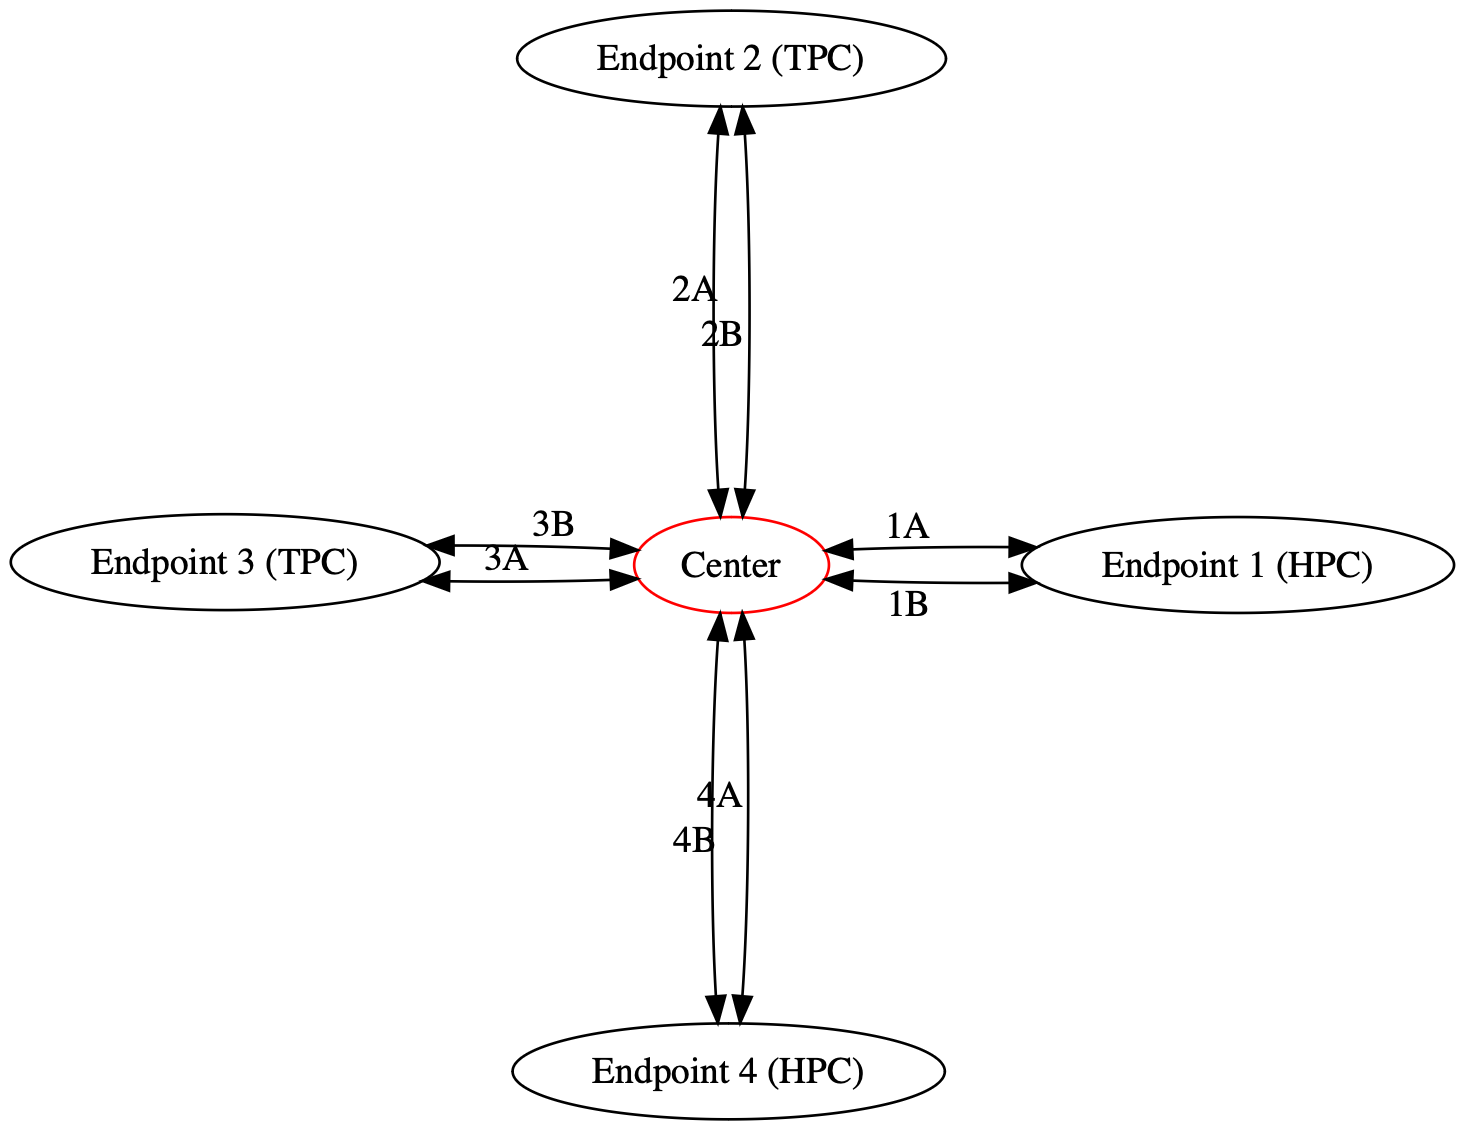
\includegraphics[width=9cm]{fig1.png}
	\centering
	\caption{Setup structure and naming of the communication channels}
    \label{fig:fig1}
\end{figure}

Figure \ref{fig:fig1} shows the structure of the test setup, where every endpoint is linked to the center through two physical 10 GbE links denoted as links \textbf{A} and \textbf{B} in the figure. The UDP communication in both directions across each of these links is measured simultaneously by a separate TestSuite process. These directions are known as \textbf{H} and \textbf{R}. Direction H refers to communication channels where the center is the sender and the endpoint is the receiver. On the other hand, direction R refers to the communication channels where the center functions as the receiver, and the endpoint serves as the sender.

The center of the star utilizes a Cocurrent iHawk computer system (refer to \textbf{ref}) that is also situated in the distributed test system. Endpoints 1 and 4 are the "High Performance PCs" and Endpoints 3 and 4 are the "Traffic PCs". The PCs located in the center and endpoints 2 and 3 are outfitted with Intel X710-T2L network cards, while those in endpoints 3 and 4 incorporate Intel X540-T2 network cards.

The settings for the network cards are those recommended for high reliability in the Intel Linux Performance Tuning Guide for the Ethernet 700 Series. These values include:

\begin{itemize}

\item Disabling of EEE (Energy Efficient Ethernet),
\item Enlarging the RX/TX ring to 4096 slots,
\item Deactivation of interrupt moderation (unless otherwise specified), and
\item Setting the UDP receive buffer to 25 MB.
\end{itemize}


The test campaigns carried out with this setup are presented below. These include long-term reliability tests, reliability tests under additional system load, investigation of the influence of CPU affinity, investigation of the influence of interrupt moderation and a comparison between the Intel X710-T2L network cards with the Intel X540-T2 network cards in the center.


\subsubsection{Results of the long-term reliability test}
The system's reliability was first tested in a long-run test with a duration of 2 hours per datagram size. Testing was conducted using datagram sizes of 80, 8900, and 65000 bytes. A cycle time of \( 0\ \mu s \) was also chosen, which corresponds to an uninterrupted transmission process. For this test, the setup described above in was used in its full configuration with all 16 communication channels.

\begin{figure}[h]
	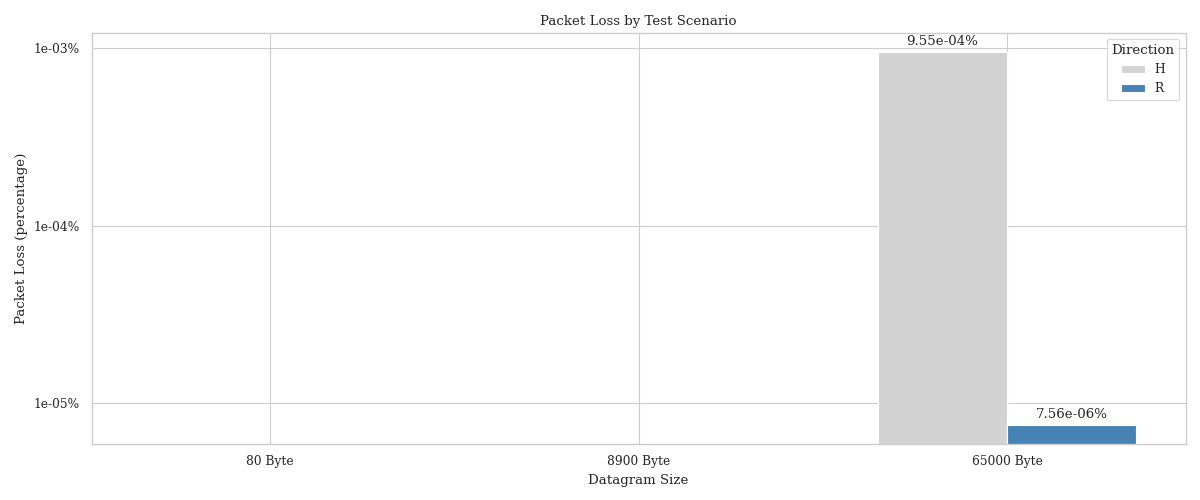
\includegraphics[width=\textwidth]{fig2.png}
	\centering
	\caption{Ratio of packet losses by datagram size and channel direction}
    \label{fig:fig2}
\end{figure}

Figure \ref{fig:fig2} illustrates the package loss ratio in this test campaign broken down by datagram size and communication direction. No packet losses occurred during the tests with datagram sizes of 80 bytes and 8900 bytes. However, packet losses were observed in both H and R directions during testing with a datagram size of 65000 byte, i.e. with fragmented UDP packets. The following section will provide a detailed examination of the system utilization, followed by a thorough discussion of the packet losses and their underlying reasons.

\paragraph*{Analysis of system utilization}

Figure \ref{fig:su1} shows the average CPU utilization at the center for all datagram sizes examined. The overall utilization for all datagram sizes was approximately 54\%. With increasing datagram size, the usage in user space declines, while kernel space usage increases. The increased use of small datagrams in the user space can be attributed to the sending of significantly more packets by the application (TestSuite) at approximately 100,000 packets per second with an 80 byte datagram size, compared to around 19,000 packets per second with a 65,000-byte datagram size. Additionally, utilization was observed in the software interrupt handling area, which involves packet processing during reception and partially during transmission. This is at its lowest with a datagram size of 8900 bytes, because fewer packets are processed (compared to 80 bytes) and no fragmentation is performed (compared to 65000 bytes).  Throughout the entire testing period, CPU usage was monitored, and no anomalies were detected; CPU utilization consistently fluctuated between \num{\pm 3}\% of the reported average utilization. The CPU load does not show any evidence of overloading of the iHawk in the center during the test. CPU utilization in the Endpoints was also considered. No overload was detected here either.

\begin{figure}[h]
	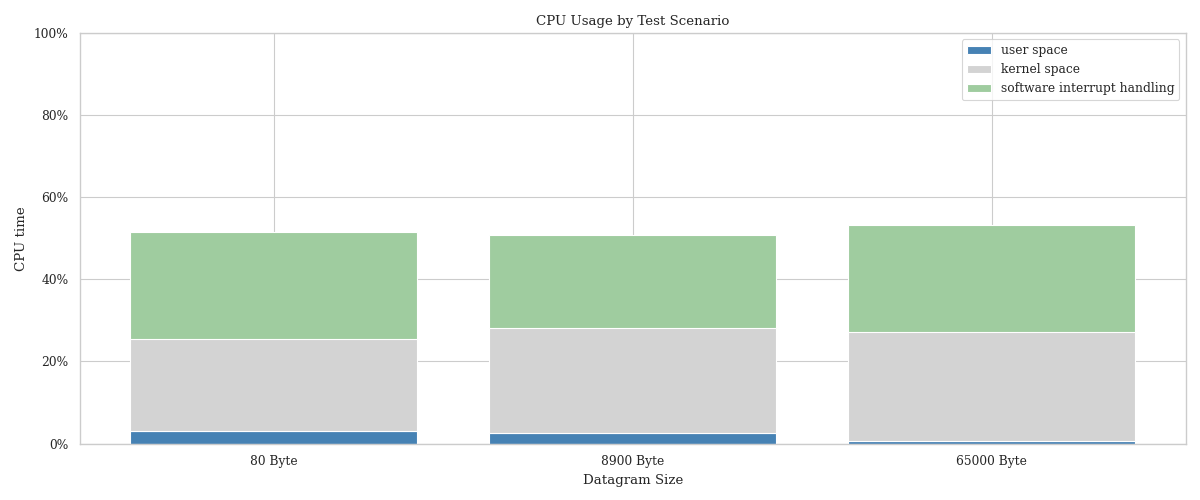
\includegraphics[width=\textwidth]{su1.png}
	\centering
	\caption{CPU usage of tests with datagram sizes of 80 bytes, 8900 bytes and 65000 bytes}
    \label{fig:su1}
\end{figure}

\begin{figure}[h]
	\includegraphics[width=\textwidth]{su3.png}
	\centering
	\caption{Data transmission rate of the utilized systems}
    \label{fig:su3}
\end{figure}

[
TODO: Sende-Datenraten in Figure \ref{fig:su3}
]



\paragraph*{Examination of package losses}
In the following, the reasons for the packet losses at 65000 bytes will be examined in more detail. As the reasons for the packet losses in the R and H directions differ, the analysis is carried out separately for each direction.

\begin{table}[h]
\centering
\begin{tabular}{||c c c||} 
 \hline
 Channel & Losses (total) & Bandwidth (net) \\ [0.5ex] 
 \hline\hline
 1A-R & 7  & 8253.4 Mbps \\ 
 1B-R & 11 & 8746.4 Mbps \\
 2A-R & 8  & 8225.9 Mbps \\
 2B-R & 8  & 8131.2 Mbps \\
 3A-R & 7  & 8121.9 Mbps \\
 3B-R & 16 & 8091.7 Mbps \\
 4A-R & 9  & 8200.9 Mbps \\
 4B-R & 9  & 8409.4 Mbps \\ [1ex] 
 \hline
\end{tabular}
\caption{ Packet losses at 65000 bytes in tests with direction R (Endpoints to Center)}
\label{table:1}
\end{table}

In the direction from the Endpoints to the Center (R), packet losses of \num{7.56e-6} \% can be observed when testing with a datagram size of 65000 Bytes. A breakdown of these losses by channel is provided in Table \ref{table:1}. It is evident that few losses occur in all communication channels in this direction. The losses are almost evenly distributed among the individual communication channels.

\begin{figure}[h]
	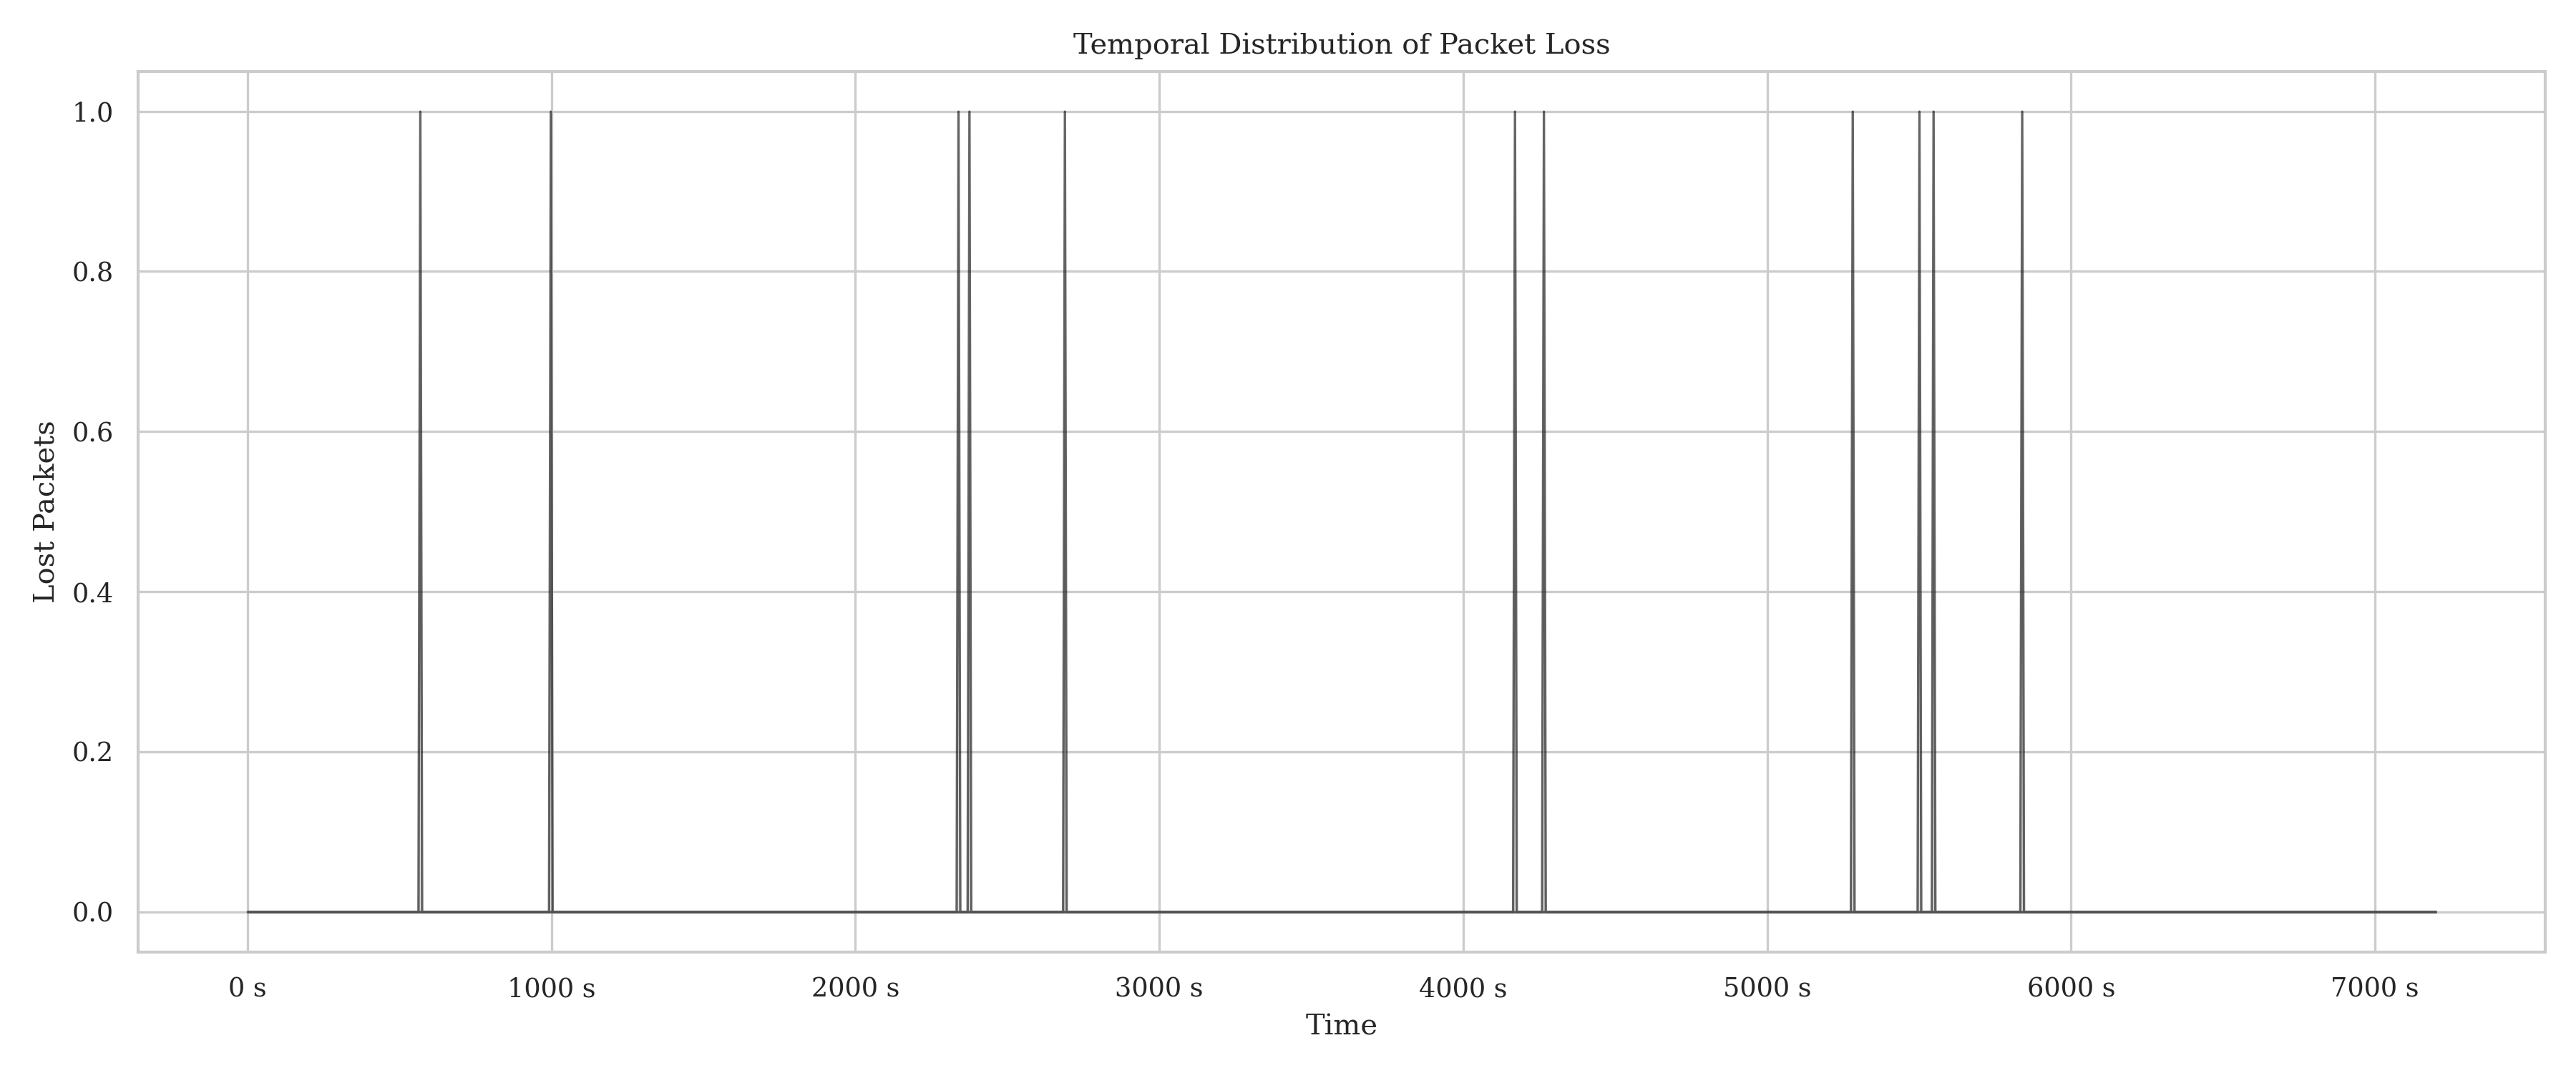
\includegraphics[width=\textwidth]{fig3.png}
	\centering
	\caption{Temporal distribution of packet losses for communication 1B-R}
    \label{fig:fig3}
\end{figure}

Figure \ref{fig:fig3} displays the temporal distribution of packet losses using channel 1B-R as an example. It is evident that the packet losses do not transpire in bursts, but instead are distributed independently across the entire test interval. This trend is also observed for the other channels.

Further investigation is required to determine the precise location and reasons for the packet losses. This is due to the fact that the statistics of the network interfaces and the network stack do not show any packet losses. This applies to both the send counters at all endpoints and the receive counters at the center. The possible causes of packet losses include losses occurring at the sender (Endpoints), losses on the route during cable transmission, and losses at the receiver (Center).

To further investigate the losses in the R direction at 65,000 bytes, test sessions of 20 minutes duration were run, gradually reducing the number of bidirectional links used until no losses occurred. Figure \ref{fig:fig4} displays the results of this investigation.

\begin{figure}[h]
	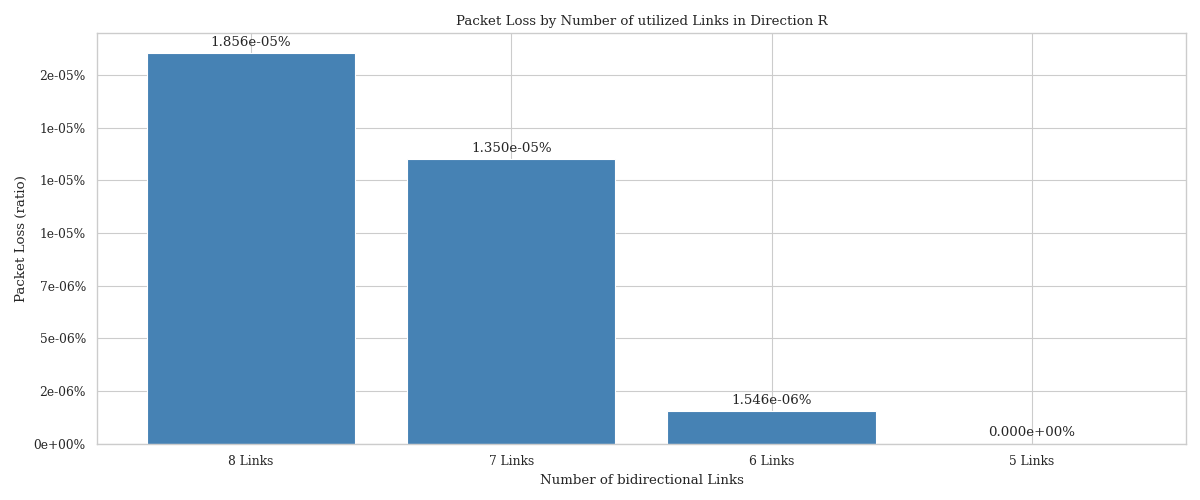
\includegraphics[width=\textwidth]{fig4.png}
	\centering
	\caption{Packet Loss by Number of utilized Links in Direction R with a datagram size of 65000 byte and a cycle time of \( 0\ \mu s \)   }
    \label{fig:fig4}
\end{figure}

The investigation indicates that no losses occur in the direction of R with the use of 5 bidirectional links. The ratio of losses in relation to the total number of packets reduces as the number of links is reduced.

During this test campaign, solely the number of links decreased, but the configuration in the TestSuite remains unchanged. Since the load on a single link remains the same, the route cannot be considered a cause for the packet losses. In the test scenario with five bidirectional links, Endpoints 1 and 4 both use their respective links, while only link A is used by Endpoint 2. Endpoint 3 is not a part of this test scenario. As the load on Endpoints 1 and 4 is the same as in the original scenario with eight links, the senders (Endpoints) cannot be considered responsible for the packet losses.

Therefore, it can be inferred that the receiver (Center) is where the packet losses occurred. The occurrence of losses exclusively with a datagram size of 65000 bytes implies a correlation with defragmentation in the network stack. One potential scenario is the overflow of the buffer allocated for defragmentation, resulting in packet losses.


\begin{table}[h]
\centering
\begin{tabular}{||c c c||} 
 \hline
 Channel & Losses (total) & Bandwidth (net) \\ [0.5ex] 
 \hline\hline
 1A-H & 0    & 9900.3 Mbps \\ 
 1B-H & 0    & 9899.8 Mbps \\
 2A-H & 0    & 9891.4 Mbps \\
 2B-H & 0    & 9893.0 Mbps \\
 3A-H & 4313 & 9890.4 Mbps \\
 3B-H & 4285 & 9892.0 Mbps \\
 4A-H & 0    & 9902.4 Mbps \\
 4B-H & 0    & 9900.8 Mbps \\ [1ex] 
 \hline
\end{tabular}
\caption{ Packet losses at 65000 bytes in tests with direction H (Center to Endpoints)}
\label{table:2}
\end{table}


The direction from the Center to Endpoints (H) experiences substantially higher packet losses (\num{9.55e-4} \%)  for datagrams sized at 65000 bytes compared to direction R (\num{7.56e-6} \%). A channel breakdown of these packet losses is included in Table \ref{table:2}, and it is noteworthy that only packet losses occur in communications with Endpoint 3.

The standard interface statistics for the relevant network interface on the sender (Center) show no losses. In contrast, the packet loss statistics for the affected receiver (Endpoint 3) show packet losses in the \codeword{rx_missed_errors} counter (see Table \ref{table:3}).


\begin{table}[h]
\centering
\begin{tabular}{||c c c c||} 
 \hline
 Interface & Channel & \codeword{rx_dropped} & \codeword{rx_missed_errors} \\ [0.5ex] 
 \hline\hline
 enp1s0f0 & 3A    & 0 & 19507 \\ 
 enp1s0f1 & 3B    & 0 & 19414 \\ [1ex] 
 \hline
\end{tabular}
\caption{Extract of standard interface statistics for Endpoint 3}
\label{table:3}
\end{table}


According to the documentation of the Linux kernel \cite{tbd}, \codeword{rx_missed_errors} signifies the number of packets which have been dropped by the computer because of inadequate space in the buffer. This suggests that the computer is unable to handle the incoming packets at the rate at which they are received at the interface, thereby leading to possible network congestion on the Endpoint 3.

The "ksoftriq" process, which handles package processing as described in chapter \textbf{ref}, was not able to handle all packets available in the network device ring-buffer before the cpu-time is up. The values for \codeword{rx_missed_errors} are higher than the recorded losses of the TestSuite. This is solely because losses only occurred at 65000 bytes, and the 65000 byte UDP packets were fragmented into 8 IP packets at the used MTU of 9000 bytes. When a fragment is lost, the entire packet is discarded.


\begin{figure}[h]
	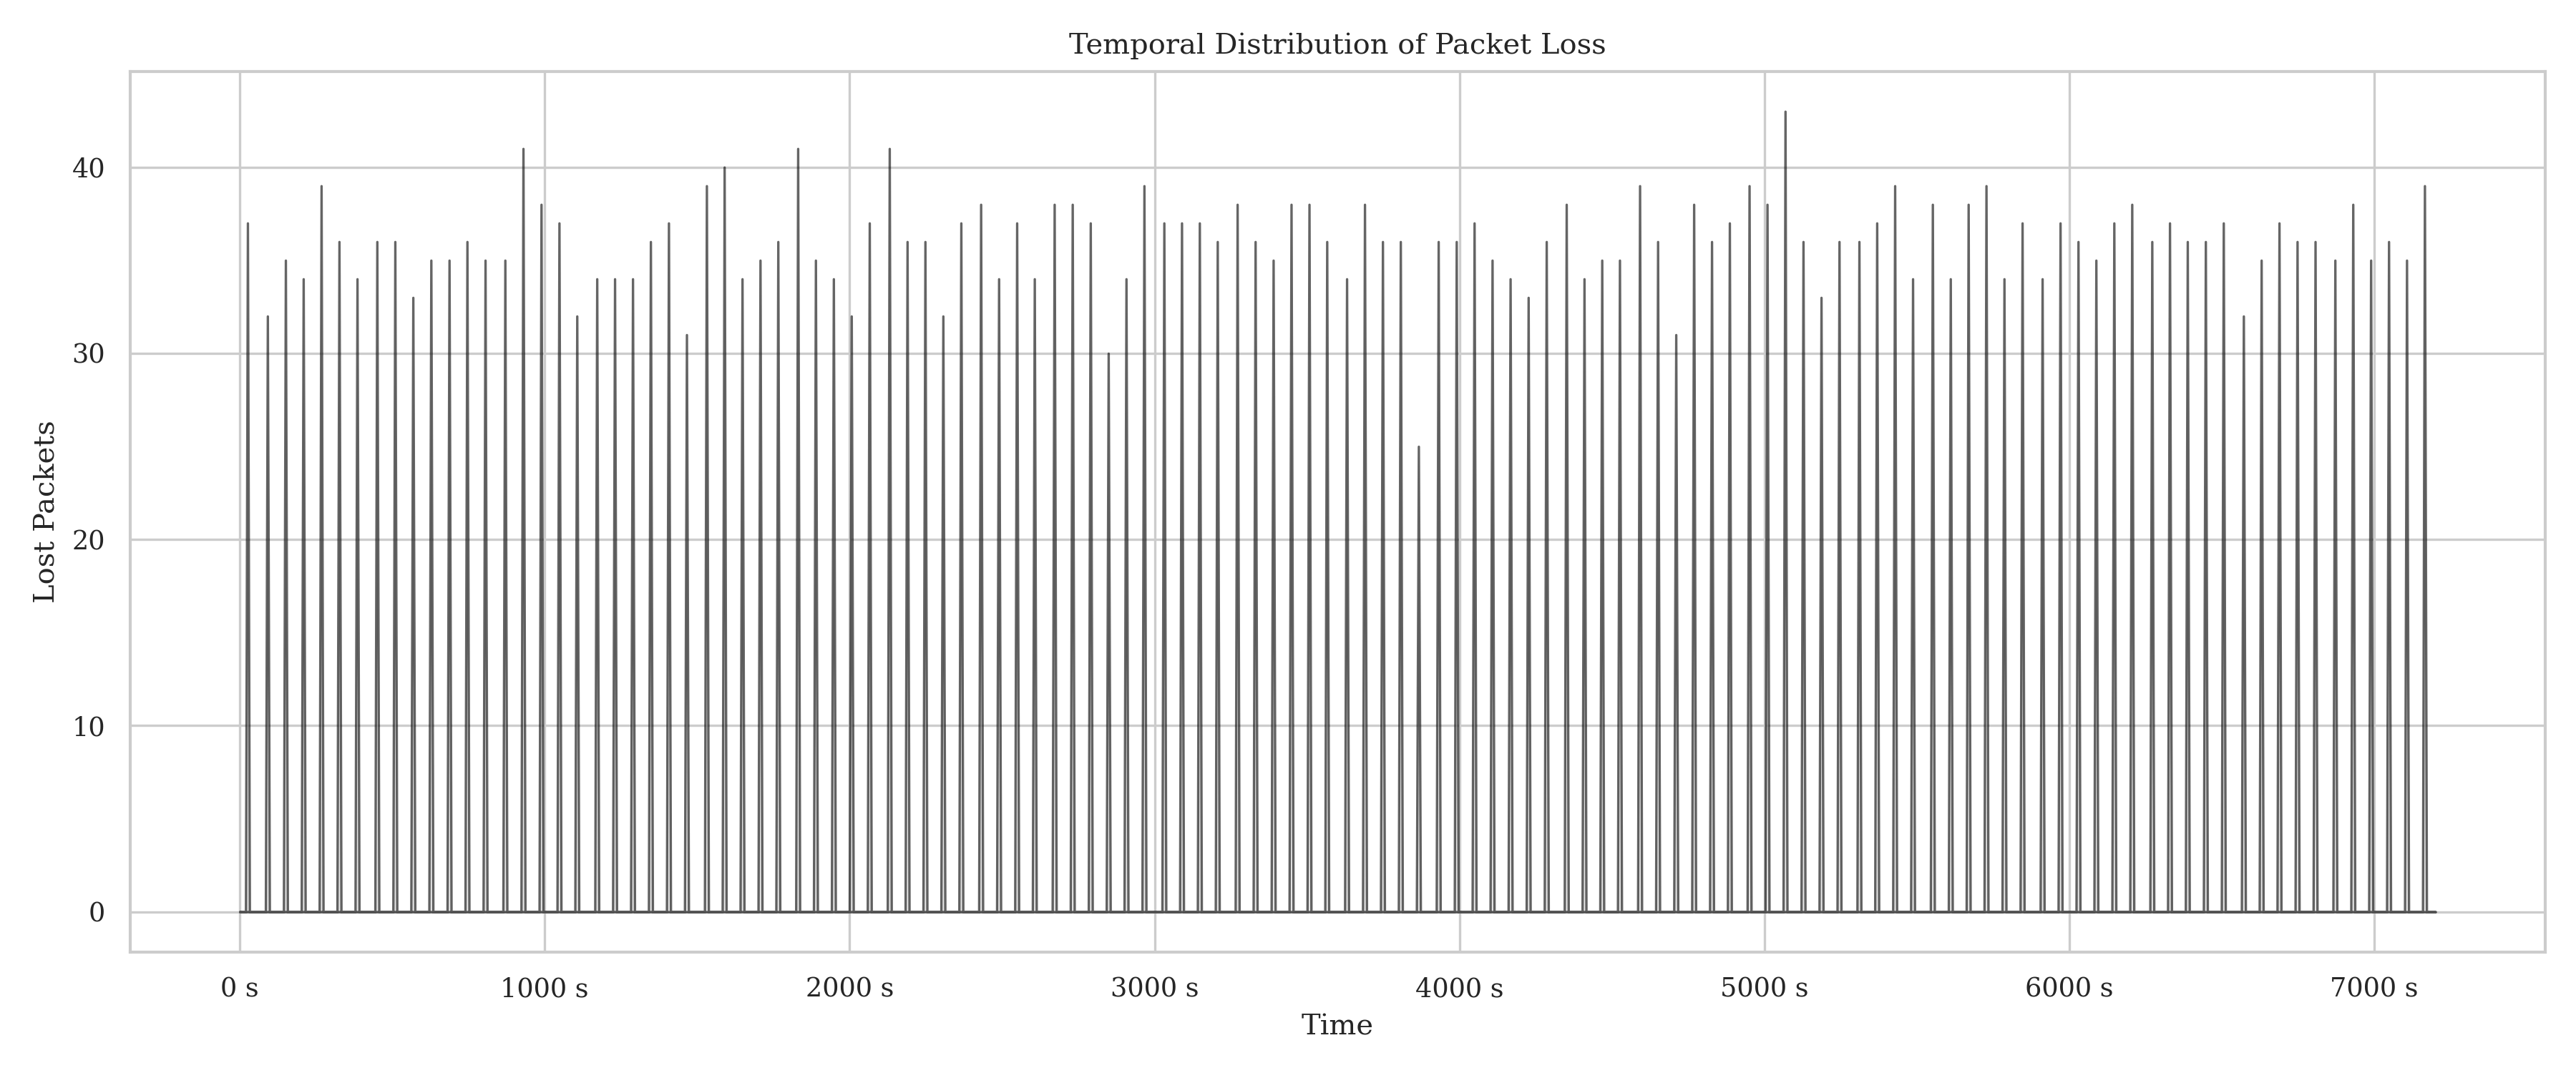
\includegraphics[width=\textwidth]{fig5.png}
	\centering
	\caption{Temporal distribution of packet losses for communication 3A-H}
    \label{fig:fig5}
\end{figure}


Figure \ref{fig:fig5} displays the temporal distribution of packet losses for communication 3A-H. The graph employs a resolution of 100,000 packets.  It is apparent that packet losses occur uniformly over time rather than in bursts. Additionally, it can be observed that losses are cyclic in nature. Upon examination of the individual query requests, it is apparent that there is packet loss of approximately 30 to 40 packets for every 900,000 packets (\num{\sim{65 }}  seconds), but no packets are lost during the intervening period. The graph for 3B-H indicates comparable results.

This confirms the hypothesis of network congestion at Endpoint 3. The endpoint cannot process incoming packets at the required speed, resulting in a buffer overflow. As a consequence, the network interface drops packets until there is enough space in the ring buffer. However, there is no indication of CPU overload as the average CPU utilization in Endpoint 3 was 41.5 \%. 

Based on the results, additional testing scenarios were conducted focusing on endpoint 3 in isolation. The test duration was set to 2 hours with the same parameters as the original testing campaign. Similar results were observed when using 2 links as in the original test. When using only 1 link, no packet loss was observed for all 3 used datagram sizes.

Another important aspect to note is that packet losses are only observed in endpoint 3. Both endpoint 2 and endpoint 3 are "Traffic-PCs". As previously explained in chapter 3.1.2, both use the same CPU and are equipped with identical network cards (Intel X540-T2) during testing, connected to the PCIe x16 slot on the motherboard. The average CPU utilization of the two computers during the test scenario was nearly identical. The primary difference between the two Traffic PCs is the motherboard used. While Traffic-PC 1 (Endpoint 2) utilizes a Gigabyte GA-Z77X-UD5H motherboard, Traffic-PC 2 (Endpoint 3) is equipped with a Gigabyte GA-Z77X-UD3H motherboard. Although the PCIe x16 slot utilized on both motherboards is directly linked to the CPUs and they both feature the same Intel X77 chip \cite{tbd}\cite{tbd}, discrepancies still exist with regards to the utilized components and cooling systems \cite{tbd}. Notably, the GA-Z77X-UD5H motherboard features enhanced cooling, which may account for the observed differences.

No losses were detected in the high-performance computers (Endpoints 1 and 4) during the testing period .



\subsubsection{Results regarding reliability with additional system load in the center}

The objective of this test campaign is to analyze the system's reliability under additional load at the center. The realistic scenario described in Section 3.2 was used as the additional system load. The number and intensity of stress-ng stressors remain the same, however, no network stressors were used because the network load is completely generated and measured by the TestSuite. The real-time priority of the stressors in the realistic load scenario is comparatively lower than that of TestSuite.

A test duration of 10 minutes was selected. Datagrams of 80, 8900, and 65000 bytes were tested to maintain consistency with the prior test. Despite packet loss in the previous scenario, a cycle time of 0µs was once again selected to evaluate the system under heavy network load. All 16 communication channels where utilized.

\begin{figure}[h]
	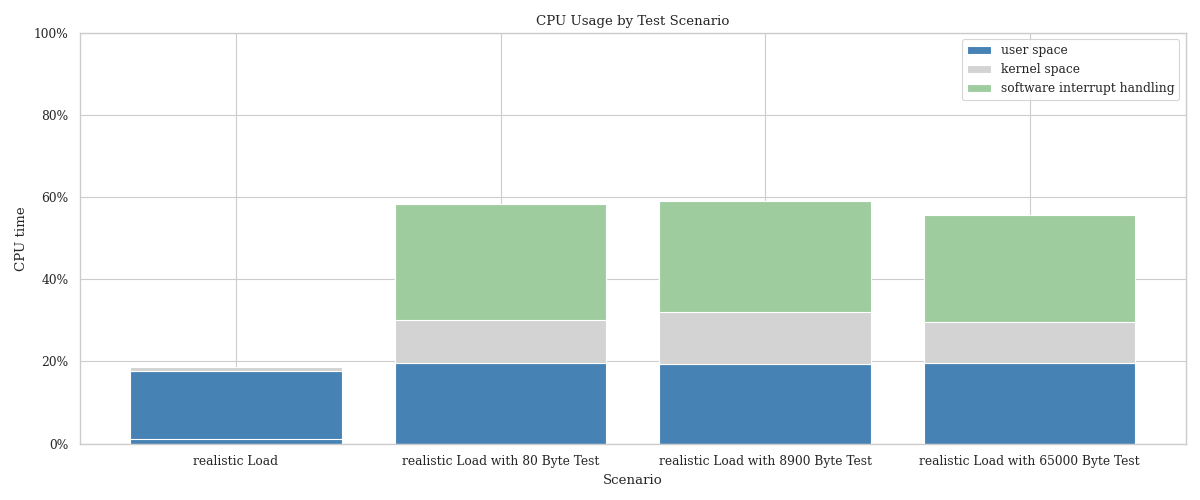
\includegraphics[width=\textwidth]{fig6.png}
	\centering
	\caption{CPU usage of realistic load and tests with datagram sizes of 80 bytes, 8900 bytes and 65000 bytes under realistic load}
    \label{fig:fig6}
\end{figure}

Figure \ref{fig:fig6} shows the average CPU utilization during this test campaign and compares it with the execution of the realistic load scenario without the execution of tests with TestSuite.

The realistic scenario utilizes 18.6\% of the system. The most of the CPU time is spent in user space (17.6\%) and 1\% of CPU time is spent in kernel space. The average CPU load during the execution of the test campaign is between 72\% and 78\% for all 3 datagram sizes. No overload situation due to the additional system load can be identified. The transmission data transfer rate at the center is also comparable to the transfer rate without additional load (Figure \ref{fig:load1}).

\begin{figure}[h]
	\includegraphics[width=\textwidth]{fig7.png}
	\centering
	\caption{Ratio of packet losses by datagram size and channel direction}
    \label{fig:fig7}
\end{figure}

Diagram \ref{fig:fig7} shows the results of the test campaign broken down by communication direction and datagram size. The results essentially correspond to the results that were also observed in the first test campaign (Diagram 1), as packet losses only occurred with a datagram size of 65000 bytes in both communication directions.

In the direction H (Center to Endpoints), packet losses were observed here, which again only occurred during communication with endpoint 3, the reasons for which have already been described in the previous section.

In direction R (Endpoints → Center), packet losses were also observed to be very low, as in the scenario without stress. The loss ratio is with \num{1.75e-5} \% slightly higher than on the scenario without additional load (\num{7.56e-6} \%), a possible explanation for this might be a variation in the exact number of packet losses, also in connection with the shorter test duration chosen for this scenario. The absolute numbers of these losses are nevertheless very low at 8 packets across all links in the direction R.


\subsubsection{Results of the CPU affinity test}
In this test campaign, the reliability impact of using CPU affinity for the sender and receiver will be investigated. CPU affinity allows processes to be bound to one or more specific CPU cores \cite{tbd}.

As previously stated in section \textbf{ref}, the iHawk's PCIe slots are directly linked to a CPU. CPU 0 is linked to slots 1 to 3, in which network cards connected to endpoints 2 and 3 are located. Meanwhile, CPU 1 is linked to slots 4 to 6, where network cards connected to endpoints 1 and 4 are located. The CPUs are connected to each other through two UPI links, each with a link frequency of 10.4 GT/s. The test campaign aims to explore potential limitations in this two-socket configuration, due to potential bottlenecks posed by the memory connection of the network cards and the connection between the CPUs.

The test campaign consisted of 2 different scenarios, each lasting 10 minutes, in which different CPU affinity options were tested. Without CPU affinity, the scheduler assigns arbitrary CPU cores to the corresponding TestSuite processes, since it has no information about which I/O devices are used by which process \cite{tbd}. In this test campaign, a scenario with enabled CPU affinity was performed. The client and server processes of TestSuite were bound to the CPU cores on the local NUMA node. This refers to CPU cores node to which the respective network card is connected. Additionally, a test was conducted with inverse CPU affinity, in which the processes of the TestSuite configured to use CPU cores of the other socket.  The network cards' Receive Side Scaling (RSS) settings were not changed on all scenarios, there are set to only use the cores on the local NUMA node by default. The size of the datagrams and the cycle time remain unchanged from the previous campaigns.

\begin{figure}[h]
	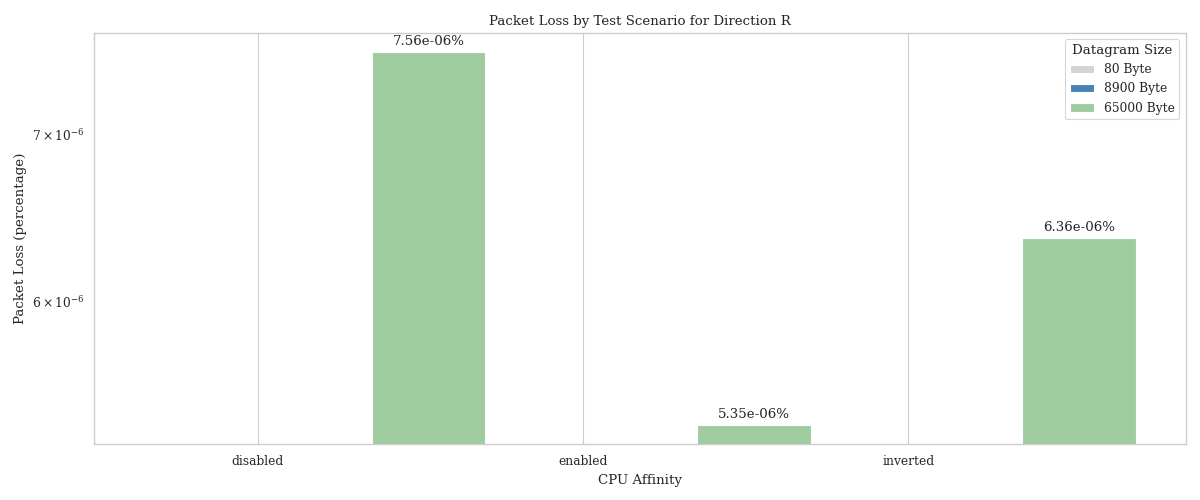
\includegraphics[width=\textwidth]{fig8.png}
	\centering
	\caption{Ratio of packet losses by datagram size for channels in direction R}
    \label{fig:fig8}
\end{figure}

Figure \ref{fig:fig8} displays the packet losses for the two CPU affinity settings selected for the R (Endpoints to Center) direction and compares them to the results with no affinity setting from a previous campaign. The packet losses in the direction H (Center to Endpoints) will not be discussed in detail here, as no particular anomalies were observed here compared to the other test campaigns. There were, again, packet losses in the communication channels from the center to endpoint 3.

Packet losses were observed with all three affinity settings in the direction of R when the datagram size was 65000 bytes, which is in connection with fragmented packets. These losses were also observed in the previous test campaigns.  The packet loss ratio varies slightly depending on the affinity settings utilized, but remains within a comparable range. These variations in the individual test scenarios result more from fluctuations in the specific number of packet losses combined with the relatively short duration of the tests. The CPU utilization of the central PC in the network are similar for all three CPU affinity choices being evaluated, and have already been described in a previous section.

\begin{figure}[h]
	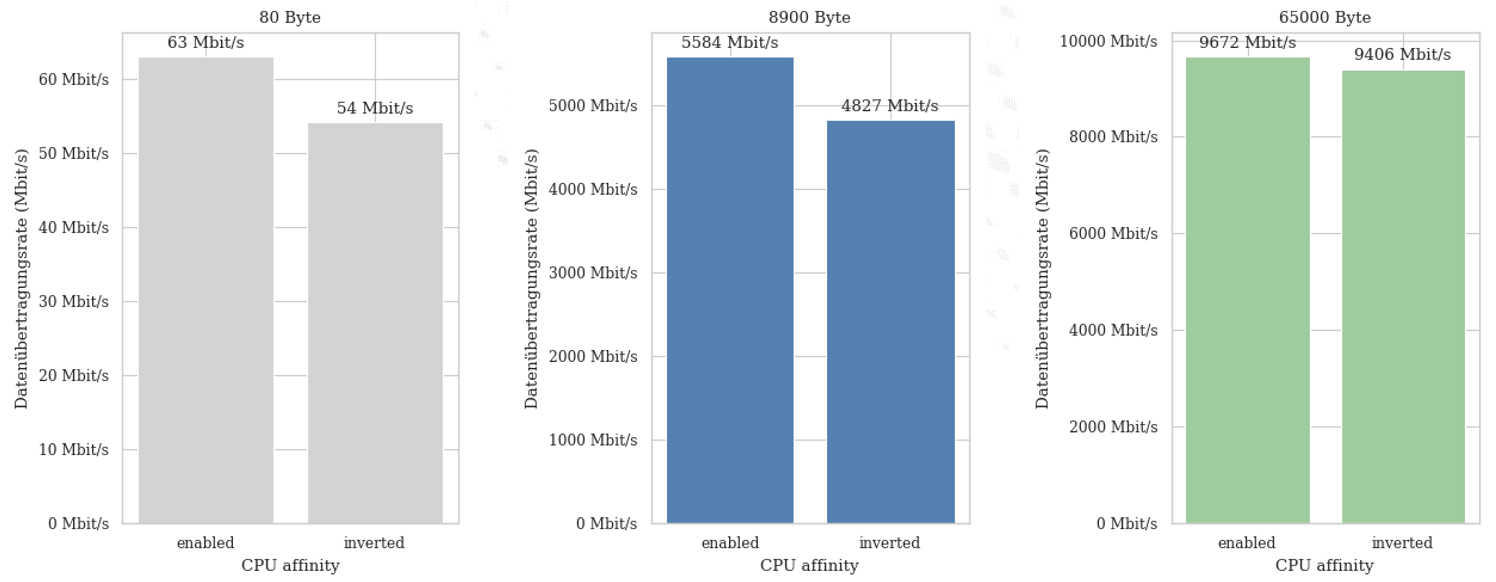
\includegraphics[width=\textwidth]{fig9.png}
	\centering
	\caption{Net transmit data rate of the center}
    \label{fig:fig9}
\end{figure}

A noticeable result of this test campaign is the difference in the center's net transmit data rates. Figure \ref{fig:fig9} compares the transmit data rates between enabled CPU affinity and inverted CPU affinity. It can be seen that for datagram sizes of 80 bytes and 8900 bytes, the send data rate in the enabled CPU affinity scenario is about 15\% higher than in the inverse CPU affinity scenario. For a datagram size of 6500 bytes, the send rate is approximately 3\% higher. The reason for the higher send data rates is that the CPU can access its local resources much faster than the other CPU. The latency of the Intel Ultra Path Interconnect, which connects the two CPU sockets, is about 130ns \cite{tbd}.

From this test campaign, it can be concluded that CPU affinity does not impact system reliability. Additionally, potential bottlenecks, such as memory connection of network cards and connection between CPUs in multi-socket systems, do not affect the reliability of a communication in a distributed test system.


\subsubsection{Investigation of the influence of interrupt moderation on the reliability and utilization of the center}

When using interrupt moderation, the network card does not generate an interrupt immediately after a packet arrives, but waits until several packets have arrived and a timeout has expired \cite{tbd}. This reduces CPU usage and is the focus of the current test campaign, which aims to examine the effect of interrupt moderation on reliability. Additionally, the center's CPU load will be evaluated. The test campaign was carried out with three datagram sizes of 80, 8900 and 65000 bytes and a duration of 5 minutes each.

Intel recommends disabling interrupt moderation in the Linux Performance Tuning Guide \cite{tbd} to achieve optimal performance and reliability, although it comes at a cost of significantly increased CPU usage. Additionally, the guide suggests timeout values of 84µs (equivalent to \num{\sim{12000}} interrupts/s) and 62µs (equivalent to \num{\sim{16000}} interrupts/s). By default, adaptive interrupt moderation is enabled, which Intel claims strikes a balance between low CPU utilization and high performance. The interrupt rate is automatically adjusted based on variables such as packet count, packet size, and connection count \cite{tbd}. Results from prior tests conducted on a "high-performance PC" situated at the center of the star revealed packet loss incidents resulted from adaptive interrupt moderation during peak usage. This means that the adaptive interrupt moderation may not be suitable for communication in the distributed test system. Nevertheless, it was included in the test campaign as a comparison. Both RX and TX interrupt moderation rates are changed in the test scenarios.

No significant differences in reliability were found among the various rates of interrupt moderation and the scenario without such moderation. Similar to the test scenario with interrupt moderation disabled, low levels of packet loss in the R direction were detected in all three variants tested. Additionally, packet losses were detected at endpoint 3. These losses also have been discussed in the previous sections.

\begin{figure}[h]
	\includegraphics[width=\textwidth]{fig10.png}
	\centering
	\caption{CPU load in the Center with different interrupt moderation settings}
    \label{fig:fig10}
\end{figure}

Figure \ref{fig:fig10} shows the CPU usage in the center with different interrupt moderation settings. It is evident that, in line with predictions, CPU utilization reaches its maximum at approximately 54\% when interrupt moderation is disabled. All three datagram sizes exhibit similar values in this case. The two interrupt moderation rates of \( 84\ \mu s \) and \( 62\ \mu s \) record equally high CPU utilization rates of around 33\%, with slightly higher values observed for \( 62\ \mu s \). However, these two test scenarios revealed significant differences in datagram sizes across the various areas. Small datagrams, particularly those of 80 bytes in the test, experience benefits from interrupt moderation. This is due to a higher amount of UDP packets being sent or received per second (\num{\sim{99000}} pps) compared to the other two datagram sizes (\num{\sim{81000}} pps for 8900 bytes and \num{\sim{19000}} pps for 65000 bytes). The use of interrupt moderation results in fewer generated interruptions and reduces CPU load.

Adaptive interrupt moderation showed differences in CPU utilization compared to a fixed moderation rate. Here, the interrupt rate is set to provide low latency or high throughput depending on the type of traffic. This procedure is detailed in the patent \cite{tbd}. For small datagrams, a low interrupt moderation rate (equivalent to a high number of interrupts per second) is selected, while for large datagrams, a high interrupt moderation rate (equivalent to a lower number of interrupts per second) is selected. This is also consistent with the CPU usage results, which are significantly higher for 80 bytes than for 8900 or 65000 bytes.

However, the interrupt moderation in connection with the selected interrupt rate also has an influence on the latency, which is considered in section \textbf{ref}.


\subsubsection{Comparison of the reliability of the Intel X710-T2L and Intel X540-T2 network cards}

The reliability of Intel X540-T2L network cards in the center of the star will be examined in this test campaign. Both network cards have two RJ45 ports and are capable of 10 GbE. The X540 chipset network cards were released in 2012 and are 7 years older than the X710 chipset network cards \cite{tbd}\cite{tbd}. Additionally, the X540s use a different driver called ixgbe. Both devices support calculating the checksum of UDP or IPv4 packets and support packet fragmentation offloading.

During testing, datagram sizes of 80 bytes, 8900 bytes, and 6500 bytes were considered, with a 0µs cycle time and a test duration of 2 hours each. The reliability results show no noticeable differences compared to the Intel X710-T2L network cards. In the R direction, a minimal number of packet losses were observed that can be attributed to the center, as previously mentioned. However, no packet losses were recorded in the H direction during the test.

Moreover, there were no notable variations in the transmission data rates of the center achieved through the utilization of Intel X540-T2 network cards and those of Intel X710-T2L network cards (as explained in section \textbf{ref}). Both cards also show a similarly CPU utilization.


\subsubsection{Insights from the tests with star topology}

Overall, packet losses were detected during the tests, but only under maximum load and in relation to fragmented packets with a size of 65,000 bytes. Thus, from a reliability perspective, the examined star topology is still suitable for a distributed test system.

Additionally, no impact was found with increased stress at the center, and the location of the CPU socket on which the send or receive process is executed. No differences in reliability were found among the different interrupt moderation rates tested, despite a noticeable difference in CPU utilization.

Furthermore, the reliability of the Intel X540-T2 network card in the center was tested. No differences to the X710-T2L were found. Therefore, the Intel X540-T2 is also suitable for use in the center of a distributed test system.










\end{document}
